%%%%%%%%%%%%%%%%%%%%%%%%%%%%%%%%%%%%%%%%%%%%%%%%%%%%%%%%%%%%%%%%%%%%%%%%%%%%%%
%
% Section file included in main project file using \input{}
%
% Assumes that LaTeX2e macros and packages defined in cg_comp.sty are
%   available
%
%%%%%%%%%%%%%%%%%%%%%%%%%%%%%%%%%%%%%%%%%%%%%%%%%%%%%%%%%%%%%%%%%%%%%%%%%%%%%%

 \section{Tempering the Classical Guitar\label{app:temp}}

 \begin{quote}
 Temperament: A compromise between the acoustic purity of theoretically exact intervals, and the harmonic discrepancies arising from their practical employment. --- Dr.\ Theo.\ Baker~\cite{ref:baker1895dmt}
 \end{quote}

Shown in \fig{shift_alhambra8p_ej45_fact_temp}, the factory guitar tuned to 12-TET shows the third string having the greatest error in tuning across the fretboard. Tuning the factory guitar to 12-TET exacts a perfect-fifth in the third string while playing a C major chord in first position. This results in the third string being too sharp (+7 cents) for the other common chords of E major (G\#), A major and D major (A). A way to reduce this error is by lowering the pitch of the third string 7 cents below 12-TET with an electronic tuner. Another more comprehensive system is to tune all the strings harmonically to the fifth string, which lowers the third string by 7 cents as well as tempering the remaining strings.

In this particular case, the ``Harmonic Tuning Method'' can be followed using these steps:
 \begin{enumerate}
  \item Begin by tuning the fifth string to A$_2 = 110$~Hz, resulting in a fifth-fret harmonic of A$_4 = 440$~Hz. (This can also be tuned by ear using an A$_4$ tuning fork).
  \item Tune that harmonic to the seventh fret harmonic of the fourth string, which is also A$_4 = 440$~Hz.
  \item Tune the seventh fret harmonic on the fifth string (330~Hz, or 0.37~Hz sharper than 12-TET E$_4$) to the fifth-fret harmonic of the sixth string.
  \item The seventh fret harmonic on the fifth string can tune the remaining fretted strings: the ninth fret on the third string, the fifth fret on the second string, and the open first string.
 \end{enumerate}

 \begin{table}[htbp]
  \centering
  \caption{\label{tbl:harmonic_tuning} Harmonic tuning methodology based on A$_4$ and E$_4$. The asterisk indicates a harmonic with a null at the designated fret.}
    \begin{tabular}{cc}
    \toprule
    Reference String/Fret &  Target String/Fret \\
    \midrule
     A$^\ast$/5 (A$_4$) & D$^\ast$/7 \\
     A$^\ast$/7 (E$_4$) & E$^\ast$/5 \\
     A$^\ast$/7 (E$_4$) & G/9 \\
     A$^\ast$/7 (E$_4$) & B/5 \\
     A$^\ast$/7 (E$_4$) & E/0 \\
    \bottomrule
    \end{tabular}
 \end{table}%

 \begin{figure}
  \centering
  \begin{subfigure}[b]{0.45\textwidth}
   \centering
   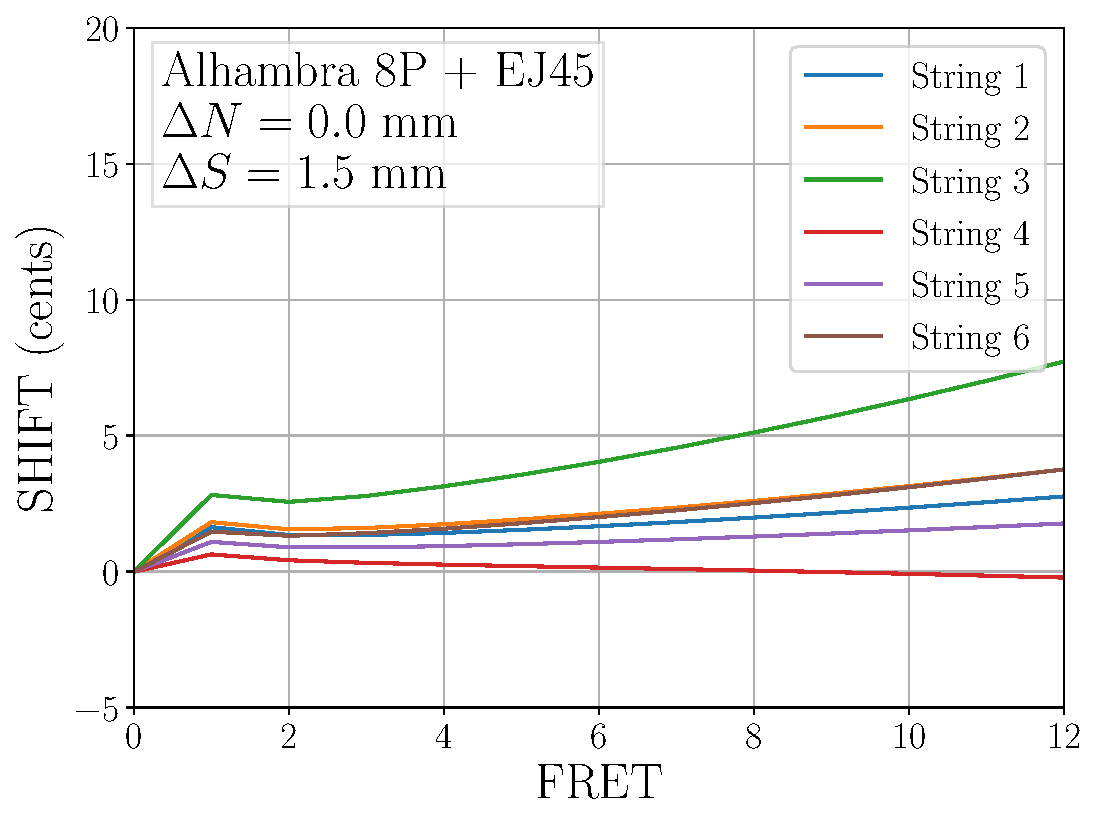
\includegraphics[width=3.25in]{figures/shift_alhambra8p_ej45_factory}
   \caption{Factory guitar --- 12-TET tuned}
   \label{fig:shift_alhambra8p_ej45_fact_temp}
  \end{subfigure}
  \hspace{0.25in}
  \begin{subfigure}[b]{0.45\textwidth}
   \centering
   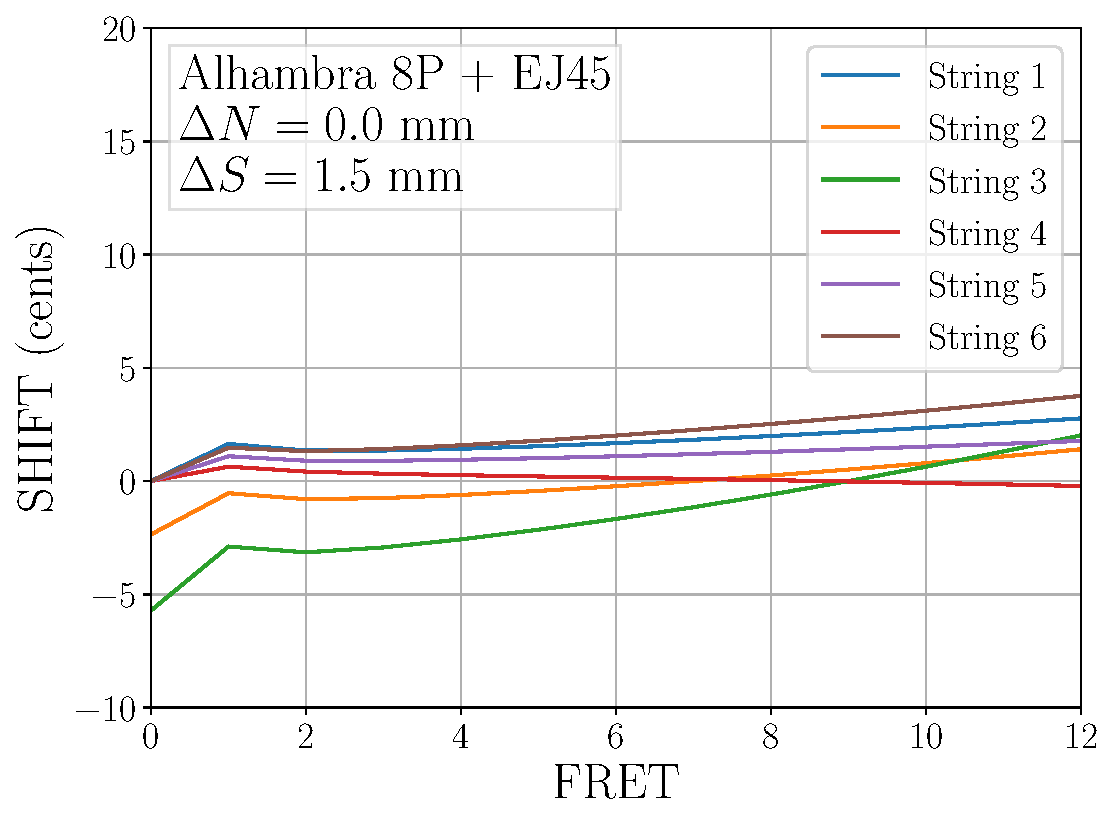
\includegraphics[width=3.25in]{figures/shift_alhambra8p_ej45_harmonic}
   \caption{Factory guitar --- harmonically tuned}
   \label{fig:shift_alhambra8p_ej45_harmonic}
  \end{subfigure}
  \caption{\label{fig:compensation_alhambra8p_ej45_temp} Frequency shift (in cents) for an Alhambra 8P guitar with normal tension nylon strings (D'Addario EJ45). Here we compare (a) the factory guitar tuned to 12-TET with (b) the same guitar harmonically tuned using the approach outlined in \tbl{harmonic_tuning}.}
 \end{figure}

 \begin{figure}
  \centering
  \begin{subfigure}[b]{0.45\textwidth}
   \centering
   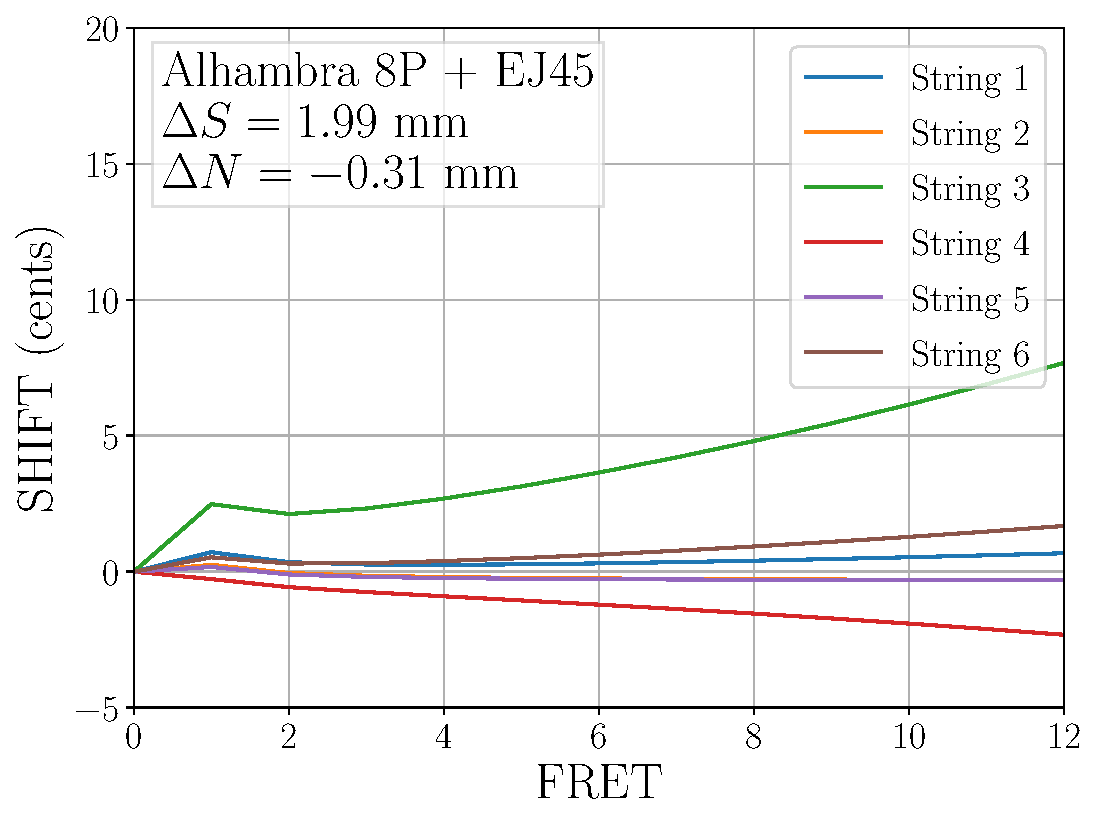
\includegraphics[width=3.25in]{figures/shift_alhambra8p_ej45_comp_x3}
   \caption{Factory guitar --- 12-TET tuned}
   \label{fig:shift_alhambra8p_ej45_comp_x3}
  \end{subfigure}
  \hspace{0.25in}
  \begin{subfigure}[b]{0.45\textwidth}
   \centering
   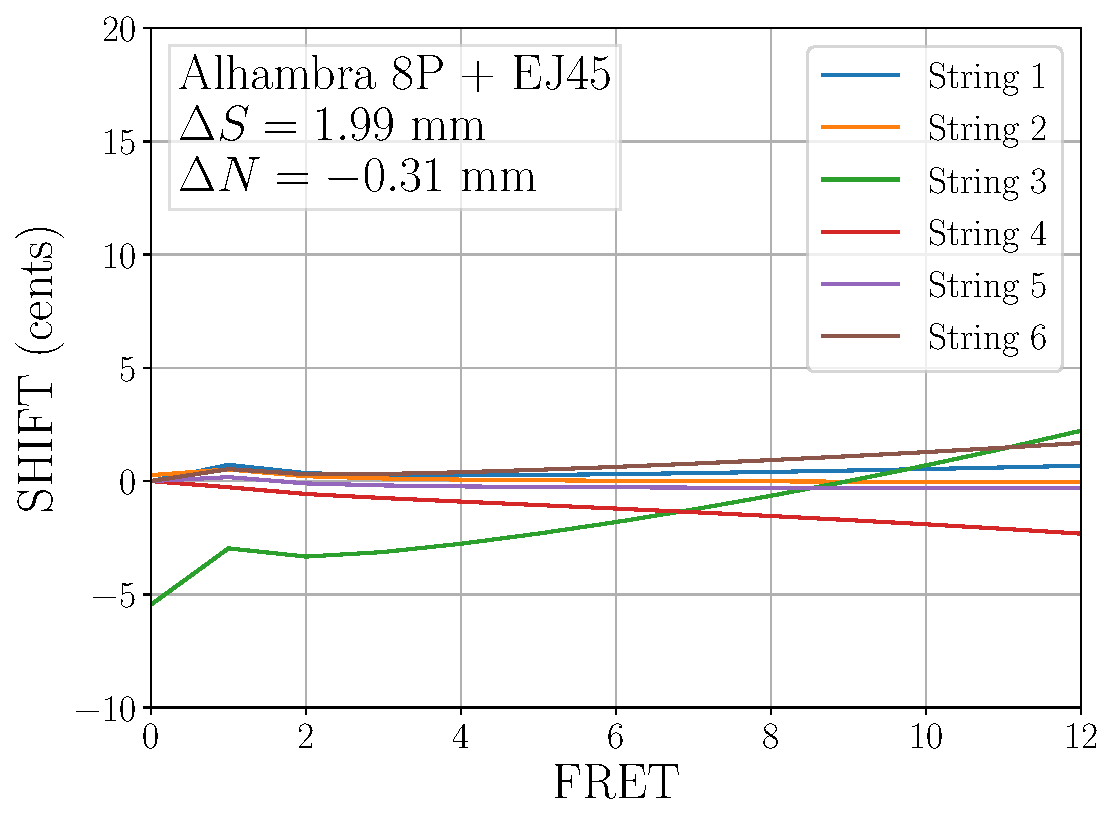
\includegraphics[width=3.25in]{figures/shift_alhambra8p_ej45_harm_x3}
   \caption{Factory guitar --- harmonically tuned}
   \label{fig:shift_alhambra8p_ej45_harm_x3}
  \end{subfigure}
  \caption{\label{fig:compensation_alhambra8p_ej45_x3} Frequency shifts (in cents) for an ``Alhambra 8P'' guitar with normal tension nylon strings (D'Addario EJ45). Instead of the factory setbacks, in (a) we set $\Delta S$ and $\Delta N$ to the mean of the corresponding column in \tbl{ej45_setbacks} \emph{neglecting the third string}. In (b), we show the same guitar harmonically tuned using the approach outlined in \tbl{harmonic_tuning}.}
 \end{figure}
